\documentclass[12pt]{article}
\usepackage[utf8]{inputenc}

\usepackage{lmodern}

\usepackage{enumitem}
\usepackage[margin=2cm]{geometry}

\usepackage{amsmath, amsfonts, amssymb}
\usepackage{graphicx}
%\usepackage{subfigure}
\usepackage{tikz}
\usepackage{pgfplots}
\usepackage{multicol}

\usepackage{comment}
\usepackage{url}
\usepackage{calc}
\usepackage{subcaption}
\usepackage[indent=0pt]{parskip}
\usepackage{animate}

\usepackage{array}
\usepackage{blkarray,booktabs, bigstrut}
\usepackage{bigints}

\pgfplotsset{compat=1.16}

% MATH commands
\newcommand{\ga}{\left\langle}
\newcommand{\da}{\right\rangle}
\newcommand{\oa}{\left\lbrace}
\newcommand{\fa}{\right\rbrace}
\newcommand{\oc}{\left[}
\newcommand{\fc}{\right]}
\newcommand{\op}{\left(}
\newcommand{\fp}{\right)}

\newcommand{\bi}{\mathbf{i}}
\newcommand{\bj}{\mathbf{j}}
\newcommand{\bk}{\mathbf{k}}
\newcommand{\bF}{\mathbf{F}}

\newcommand{\mR}{\mathbb{R}}

\newcommand{\ra}{\rightarrow}
\newcommand{\Ra}{\Rightarrow}

\newcommand{\sech}{\mathrm{sech}\,}
\newcommand{\csch}{\mathrm{csch}\,}
\newcommand{\curl}{\mathrm{curl}\,}
\newcommand{\dive}{\mathrm{div}\,}

\newcommand{\ve}{\varepsilon}
\newcommand{\spc}{\vspace*{0.5cm}}

\DeclareMathOperator{\Ran}{Ran}
\DeclareMathOperator{\Dom}{Dom}

\newcommand{\exo}[1]{\noindent\textcolor{red}{\fbox{\textbf{Problem {#1}}}\hrulefill}\\}
\newcommand{\qu}[4]{\noindent\textcolor{#4}{\fbox{\textbf{Section {#1} | Problem {#2}}} \hrulefill{{\fbox{\textbf{{#3} Points}}}}\\}}

\newcommand{\semester}{Spring 2023}

\newcommand{\CVup}{%

\begin{tikzpicture}
\draw[black, <->, >=latex] (-0.33, 0.5) .. controls (-0.125, 0) and (0.125, 0) .. (0.33, 0.5);
\end{tikzpicture}}

\newcommand{\CVupInc}{%
\begin{tikzpicture}
\draw[black, ->, >=latex] (0,0) .. controls (0.2, 0) and (0.4, 0.2) .. (0.5, 0.5);
\end{tikzpicture}}

\newcommand{\CVupDec}{%
\begin{tikzpicture}[rotate=270]
\draw[black, ->, >=latex] (0,0) .. controls (0.2, 0) and (0.4, 0.2) .. (0.5, 0.5);
\end{tikzpicture}}

\newcommand{\CVdown}{%
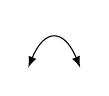
\begin{tikzpicture}
\draw[black, <->, >=latex] (-0.33, -0.5) .. controls (-0.125, 0) and (0.125, 0) .. (0.33, -0.5);
\end{tikzpicture}}

\newcommand{\CVdownInc}{%
\begin{tikzpicture}
\draw[black, ->, >=latex] (-0.5, -0.5) .. controls (-0.5, -0.3) and (-0.5, -0.1) .. (0,0);
\end{tikzpicture}}

\newcommand{\CVdownDec}{%
\begin{tikzpicture}[rotate=-90]
\draw[black, ->, >=latex] (-0.5, -0.5) .. controls (-0.5, -0.3) and (-0.5, -0.1) .. (0,0);
\end{tikzpicture}}

\begin{document}
	\noindent \hrulefill \\
	MATH-241 \hfill Pierre-Olivier Paris{\'e}\\
	Solutions Section 3-4 \hfill \semester \\\vspace*{-1cm}
	
	\noindent\hrulefill
	
	\spc
	
	\exo{8}
	\\
	We factor the greatest power of $x$:
		\begin{align*}
		\frac{9x^3 + 8x - 4}{3 - 5x + x^3} = \frac{x^3 (9 + 8/x^2 - 4/x^3)}{x^3 (3/x^3 - 5/x^2 + 1)} = \frac{9 + 8/x^2 - 4/x^3}{3/x^3 - 5/x^2 + 1} .
		\end{align*}
	We have
		\begin{align*}
		\lim_{x \ra \infty} 9 + 8/x^2 - 4/x^3 = \lim_{x \ra \infty} 9 + 8 \lim_{x \ra \infty} 1/x^2 - 4 \lim_{x \ra \infty} 1/x^3 = 9 + 8\times 0 - 4 \times 0 = 9 
		\end{align*}
	and
		\begin{align*}
		\lim_{x \ra \infty} 3/x^3 - 5/x^2 + 1 = 3 \lim_{x \ra \infty} 1/x^3 - 5 \lim_{x \ra \infty} 1/x^2 + \lim_{x \ra \infty}
		 1 = 3 \times 0 - 5 \times 0 + 1 = 1 .
		\end{align*}
	So, we obtain
		\begin{align*}
		\lim_{x \ra \infty} \frac{9x^3 + 8x - 4}{3 - 5x + x^3} = \lim_{x \ra \infty} \frac{9 + 8/x^2 - 4/x^3}{3/x^3 - 5/x^2 + 1} = \frac{\lim_{x \ra \infty} 9 + 8/x^2 - 4/x^3}{\lim_{x \ra \infty} 3/x^3 - 5/x^2 + 1} = \frac{9}{1} = 9  
		\end{align*}
	and then
		\begin{align*}
		\lim_{x \ra \infty} \sqrt{\frac{9x^3 + 8x - 4}{3 - 5x + x^3}} = \sqrt{\lim_{x \ra \infty} \frac{9x^3 + 8x - 4}{3 - 5x + x^3}} = \sqrt{9} = 3 .
		\end{align*}
		
	\spc
	
	\exo{12}
	\\
	Factoring $x^3$, we have
		\begin{align*}
		\frac{4x^3 + 6x^2 - 2}{2x^3 - 4x + 5} = \frac{4 + 6/x - 2/x^3}{2 - 4/x^2 + 5/x^3}
		\end{align*}
	Using the fact that $\lim_{x \ra -\infty} \frac{1}{x^r} = 0$, we obtain
		\begin{align*}
		\lim_{x \ra -\infty} \Big( 4 + \frac{6}{x} - \frac{2}{x^3} \Big) = 4 \quad \text{ and } \quad \lim_{x \ra -\infty} \Big( 2 - \frac{4}{x^2} + \frac{5}{x^3} \Big) = 2 .
		\end{align*}
	By the quotient rule, we see that
		\begin{align*}
		\lim_{x \ra -\infty} \frac{4x^3 + 6x^2 - 2}{2x^3 - 4x + 5} = \frac{4 + 6/x - 2/x^3}{2 - 4/x^2 + 5/x^3} = \frac{4}{2} = 2 .
		\end{align*}
		
	\spc
	
	\exo{14}
	\\
	Factoring $t^{3/2}$, we have
		\begin{align*}
		\frac{t - t^{3/2}}{2t^{3/2} + 3t - 5} = \frac{1/t^{1/2} - 1}{2 + 3/t^{1/2} - 5/t^{3/2}} .
		\end{align*}
	Using the fact that $\lim_{t \ra \infty} \frac{1}{t^r} = 0$, we obtain
		\begin{align*}
		\lim_{t \ra \infty} \Big( \frac{1}{t^{1/2}} - 1 \Big) = -1 \quad \text{ and } \quad \lim_{t \ra \infty} \Big( 2 + \frac{3}{t^{1/2}} - \frac{5}{t^{3/2}} \Big) = 2 .
		\end{align*}
	By the quotient rule, we see that
		\begin{align*}
		\lim_{t \ra \infty} \frac{t - t^{3/2}}{2t^{3/2} + 3t - 5} = \frac{-1}{2} .
		\end{align*}				
		
	\spc
	
	\exo{16}
	\\
	Factoring $x^4$, we see that
		\begin{align*}
		\sqrt{x^4 + 1} = \sqrt{x^4} \sqrt{1 + 1/x^4}
		\end{align*}
	Since $x \ra \infty$, we must have that $x > 0$ eventually and therefore $\sqrt{x^4} = x^2$. Then, we can write
		\begin{align*}
		\frac{x^2}{\sqrt{x^4 + 1}} = \frac{1}{\sqrt{1 + 1/x^4}} .
		\end{align*}
	Using the fact that $\lim_{x \ra \infty} \frac{1}{x^r} = 0$, we see that
		\begin{align*}
		\lim_{x \ra \infty} \Big( 1 + \frac{1}{x^4} \Big) = 1
		\end{align*}
	and by the root law for limits, we conclude that
		\begin{align*}
		\lim_{x \ra \infty} \sqrt{1 + \frac{1}{x^4}} = 1 .
		\end{align*}
	By the quotient law, we obtain
		\begin{align*}
		\lim_{x \ra \infty} \frac{x^2}{\sqrt{x^4 + 1}} = \frac{1}{1} = 1 .
		\end{align*}
		
	\spc
	
	\exo{18}
	\\
	We have
		\begin{align*}
		\sqrt{1 + 4x^6} = \sqrt{x^6 (1/x^6 + 4)} = |x|^3 \sqrt{1/x^6 + 4} .
		\end{align*}
	Now, since $x < 0$, we have $|x| = -x$ and so
		\begin{align*}
		\sqrt{1 + 4x^6} = -x^3 \sqrt{1/x^6 + 4} .
		\end{align*}
	Then, we can rewrite the limit and compute it:
		\begin{align*}
		\lim_{x \ra -\infty} \frac{\sqrt{1 + 4x^6}}{2 - x^3} = \lim_{x \ra -\infty} \frac{-x^3 \sqrt{1/x^6 + 4}}{x^3 (2/x^3 - 1)} = \lim_{x \ra -\infty} -\frac{\sqrt{1/x^6 + 4}}{2/x^3 - 1} = - \frac{\sqrt{\lim_{x \ra -\infty} 1/x^6 + 4}}{\lim_{x \ra -\infty} 2/x^3 - 1} = 2 .
		\end{align*}
		
	\spc
	
	\exo{21}
	\\
	We multiply by the conjugate:
		\begin{align*}
		(\sqrt{9x^2 + x} - 3x) \Big( \frac{\sqrt{9x^2 + x} + 3x}{\sqrt{9x^2 + x} + 3x} \Big) = \frac{x}{\sqrt{9x^2 + x} + 3x}
		\end{align*}
	and then factor $x$:
		\begin{align*}
		\frac{x}{\sqrt{9x^2 + x} + 3x} = \frac{x}{\sqrt{x^2} \sqrt{9 + 1/x} + 3x} .
		\end{align*}
	Since we are taking the limit as $x \ra \infty$, we have $\sqrt{x^2} = x$. Therefore,
		\begin{align*}
		\lim_{x \ra \infty} (\sqrt{9x^2 + x} - 3x) = \lim_{x \ra \infty} \frac{x}{x \sqrt{9 + 1/x} + 3x} = \lim_{x \ra \infty} \frac{1}{\sqrt{9 + 1/x} + 3} .
		\end{align*}
	Since $\lim_{x \ra \infty} \frac{1}{x} = 0$, then by the rule for limits, we get
		\begin{align*}
		\lim_{x \ra \infty} (\sqrt{9x^2 + x} - 3x) = \frac{1}{\sqrt{9} + 3} = \frac{1}{6} .
		\end{align*}
		
	\spc
	
	\exo{22}
	\\
	Since $x \ra -\infty$, we have that $x < 0$ eventually. Let's multiply by the conjugate:
		\begin{align*}
		\big( \sqrt{4x^2 + 3x} + 2x \big) \Big( \frac{\sqrt{4x^2 + 3x} - 2x}{\sqrt{4x^2 - 3x} - 2x} \Big) = \frac{4x^2 + 3x - 4x^2}{ \sqrt{4x^2 + 3x} - 2x} = \frac{3x}{\sqrt{4x^2 + 3x} - 2x} .
		\end{align*}
	Factoring $x^2$ in the root, we find
		\begin{align*}
		\sqrt{4x^2 + 3x} = \sqrt{x^2}\sqrt{4 + 3/x} 
		\end{align*}
	and since $x < 0$, we have $\sqrt{x^2} = -x$. This means we can rewrite the above expression as followed:
		\begin{align*}
		\sqrt{4x^2 + 3x} = - x\sqrt{4 + 3/x} .
		\end{align*}
	Replacing this last expression in the quotient above, we find out that
		\begin{align*}
		\sqrt{4x^2 + 3x} + 2x = \frac{3}{-\sqrt{4 + 3/x} - 2} .
		\end{align*}
	We therefore see that
		\begin{align*}
		\lim_{x \ra -\infty} \Big( -\sqrt{4 + \frac{3}{x}} - 2 \Big) = -4 .
		\end{align*}
	Therefore, we obtain
		\begin{align*}
		\lim_{x \ra -\infty} \frac{3}{\sqrt{4 + 3/x} - 2} = \frac{3}{-4} = -\frac{3}{4} .
		\end{align*}
		
	\spc
	
	\exo{30}
	\\
	We factor $x^2$:
		\begin{align*}
		x^2 - x^4 = x^2 (1 - x^2) .
		\end{align*}
	Therefore, since $\lim_{x \ra \infty} x^2 = \infty$ and $\lim_{x \ra \infty} (1 - x^2) = -\infty$, we obtain
		\begin{align*}
		\lim_{x \ra \infty} (x^2 - x^4) = \lim_{x \ra \infty} x^2 \lim_{x \ra \infty} (1 - x^2) = \infty (-\infty) = -\infty .
		\end{align*}
		
	\spc
	
	\exo{40}
	\\
	We first compute the limit at $\infty$. Since $x \ra \infty$, the variable $x$ will be eventually positive and so $\sqrt{x^2} = x$. Then, we can write
		\begin{align*}
		\frac{x - 9}{\sqrt{4x^2 + 3x + 2}} = \frac{1 - 9/x}{\sqrt{4 + 3/x + 2/x^2}} .
		\end{align*}
	We then find, by the quotient rule and the root rule,
		\begin{align*}
		\lim_{x \ra \infty} \frac{1 - 9/x}{\sqrt{4 + 3/x + 2/x^2}} = \frac{1}{\sqrt{4}} = \frac{1}{2} .
		\end{align*}
	So $y = 1/2$ is an HA at $\infty$.
	
	Finally, we compute the limit at $-\infty$. Since $x \ra -\infty$, the variable $x$ will eventually be negative and so $\sqrt{x^2} = -x$. We then can write
		\begin{align*}
		\frac{x - 9}{\sqrt{4x^2 + 3x + 2}} = -\frac{1 - 9/x}{\sqrt{4 + 3/x + 2/x^2}}  .
		\end{align*}
	We then find, by the quotient rule and the root rule,
		\begin{align*}
		\lim_{x \ra \infty}- \frac{1 - 9/x}{\sqrt{4 + 3/x + 2/x^2}} = \frac{1}{\sqrt{4}} = -\frac{1}{2} .
		\end{align*}
	So $y = -1/2$ is an HA at $-\infty$.
	
	\spc
	
	\exo{46}
	\\
	We need the function to have a non-zero numerator and a zero denominator at $x = 1$ and $x = 3$. A good function for that would be
		\begin{align*}
		\frac{1}{(x - 1)(x-3)} .
		\end{align*}
		
	This last expression, however, does not have a horizontal asymptote $y = 1$ because
		\begin{align*}
		\lim_{x \ra \infty} \frac{1}{(x - 1)(x - 3)} = 0
		\end{align*}
	and
		\begin{align*}
		\lim_{x \ra -\infty} \frac{1}{(x - 1) (x - 3)} = 0 .
		\end{align*}
	To change this, we can add $1$ to the previous expression. The desire function is therefore
		\begin{align*}
		f(x) = 1 + \frac{1}{(x - 1)(x - 3)} .
		\end{align*}
	
	\spc
	
	\exo{63}
	\\
	We will use the Squeeze Theorem. First, we have
		\begin{align*}
		\lim_{x \ra \infty} \frac{4x - 1}{x} = 4 .
		\end{align*}	
	Secondly, we have
		\begin{align*}
		\lim_{x \ra \infty} \frac{4x^2 + 3x}{x^2} = 4 .
		\end{align*}
	
	Therefore, the function $f$ is squeeze between two functions that have $4$ as their limit at $\infty$. Using the Squeeze Theorem, we conclude that 
		\begin{align*}
		\lim_{x \ra \infty} f (x) = 4 .
		\end{align*}	
		
	
\end{document}